\chapter{August 2015}
        \section{August 28th/29th, 2015}
    		I've been once again revisiting the \index{nRF24L01+}\hyperref[sec:nRF24L01+]{nRF24L01+} modules, attempting to finish the drivers that I've been writing for the \index{Propeller Chip}Propeller chip. On top of that I've been cram-learning \index{C}C. In the future I may rewrite these drivers for the propeller chip in C using the \index{PropGCC}PropGCC compiler. Random side note, I've found the concept and implementation of \index{linked lists}linked lists fascinating - and have ideas on how I can use such stuff on the propeller platform.\\
    		
    		For those at home who've just tuned in, I have a few cheap rf modules that I'm looking at using in the performance. I have yet to \index{reliably}reliably implement the drivers for them.\\
    		
    		Progress has been slow over the last two days because I haven't been working on this code for a while I have to get back into the same "mindset" again. It's 11:25PM on the 29th, and I'm starting to make some positive \index{progress}progress.\\
    		
            \index{SPI}
            \index{nRF24L01+}
    		\centerline{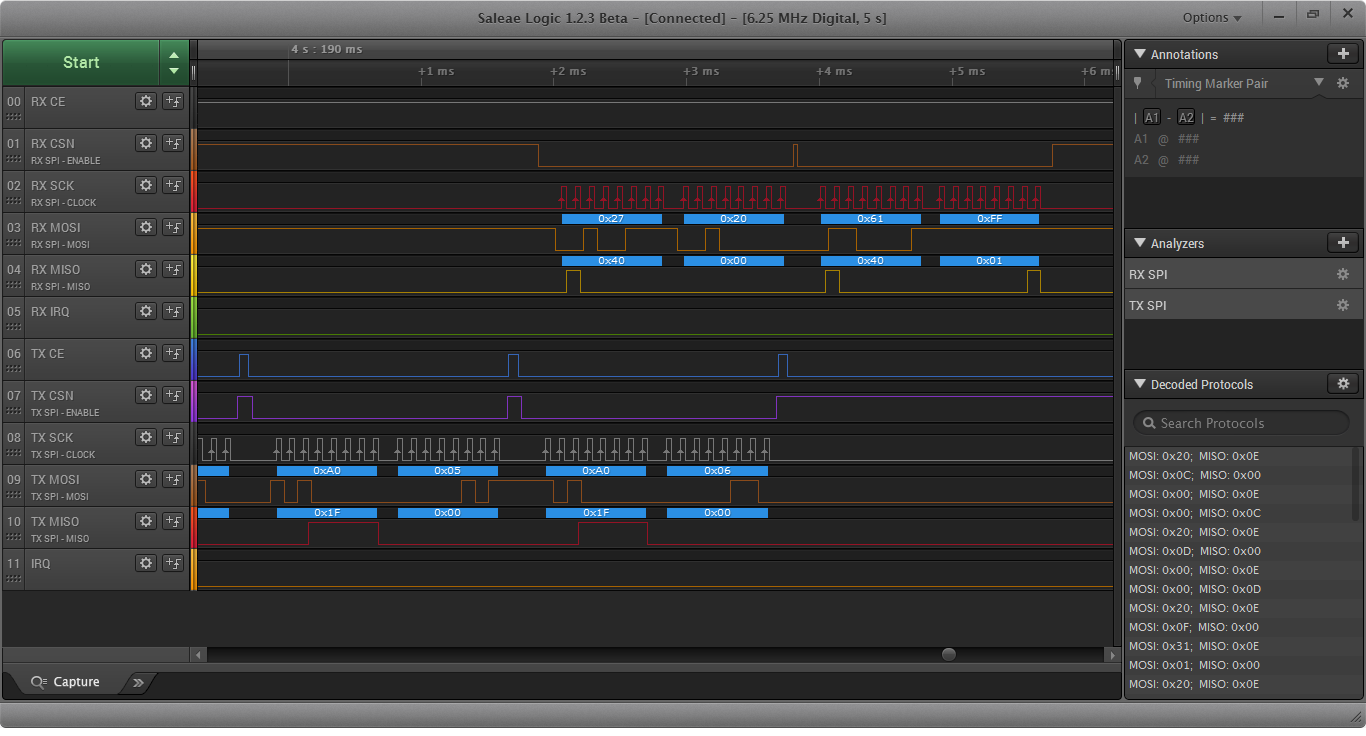
\includegraphics[width=0.75\linewidth]{images/nRF_SPI}}
    		\vspace{10pt}
    			
    		The main difficulty has been remembering to send the correct \index{byte} sequences to properly initialize the \index{nRF24L01+}\hyperref[sec:nRF24L01+]{nRF24L01+} modules. I've found that the following bytes work well:\\
    		
    		\centerline{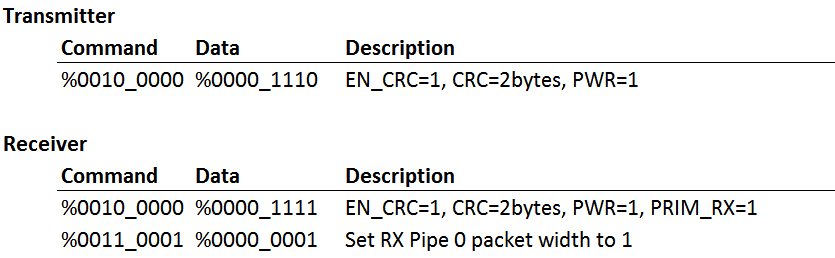
\includegraphics[width=\linewidth]{images/nRF_Protocol}}
    		\vspace{10pt}
    		
    		Previously I was having difficulties with the receiver only picking up one packet before stopping receiving - unknown reason. I reverted back to some old code from \hyperref[Git]{GitHub}\index{GitHub} for a retry - everything working so far.\\
    		
    		Now I appear to be having difficulty picking up new \index{packet}packets - the first \index{packet}packet (0x01) keeps on repeating for whatever reason - perhaps it's not deleting it from the \index{FIFO}FIFO \index{buffer}buffer when I read it.\\
    		
    		Another issue encountered was that between code changes I was only restarting the \index{MCU}MCU, not the \index{nRF24L01+}\hyperref[sec:nRF24L01+]{nRF24L01+} modules (meaning that they kept all the old data in their \index{buffers}buffers, old settings, etc). I needed a way to switch the power of both \index{MCU}MCUs on and off at the same time. In the past I've simply flicked both switches of both MCUs at the same time (before recording data using the \index{logic analyzer}Logic Analyzer). Because of limited resources, this wasn't an issue.\\
    		
    		To combat this issue I drew \index{power}power from the board with the \index{switch}switch, and fed it into the 5V rail on the other board through a \index{servo}servo header that I had previously built into that board. This solves the issue allowing for me to capture all the data for both the \index{transmitter}transmitter and \index{receiver}receiver on the \index{logic analyzer}logic analyzer cleanly.\\
    		
    	\section{August 30th, 2015}
    		I've been continuing work on the \index{nRF24L01+}\hyperref[sec:nRF24L01+]{nRF24L01+} modules today. I have found that with both Auto Retransmit, and Auto Ack left to default on the \index{transmitter}transmitter, I get 1 \index{byte}byte received on the \index{receiver}receiver, however when I disable both Auto Ack and Auto Retransmit, I do not.\\
    		
    		I define packet reception as \index{IRQ}IRQ dropping low on the RX end. I've been doing some playing around and it would appear that when Auto Ack is left to default, and Auto Retransmit is turned off, the system works fine.\\
    		
    		\centerline{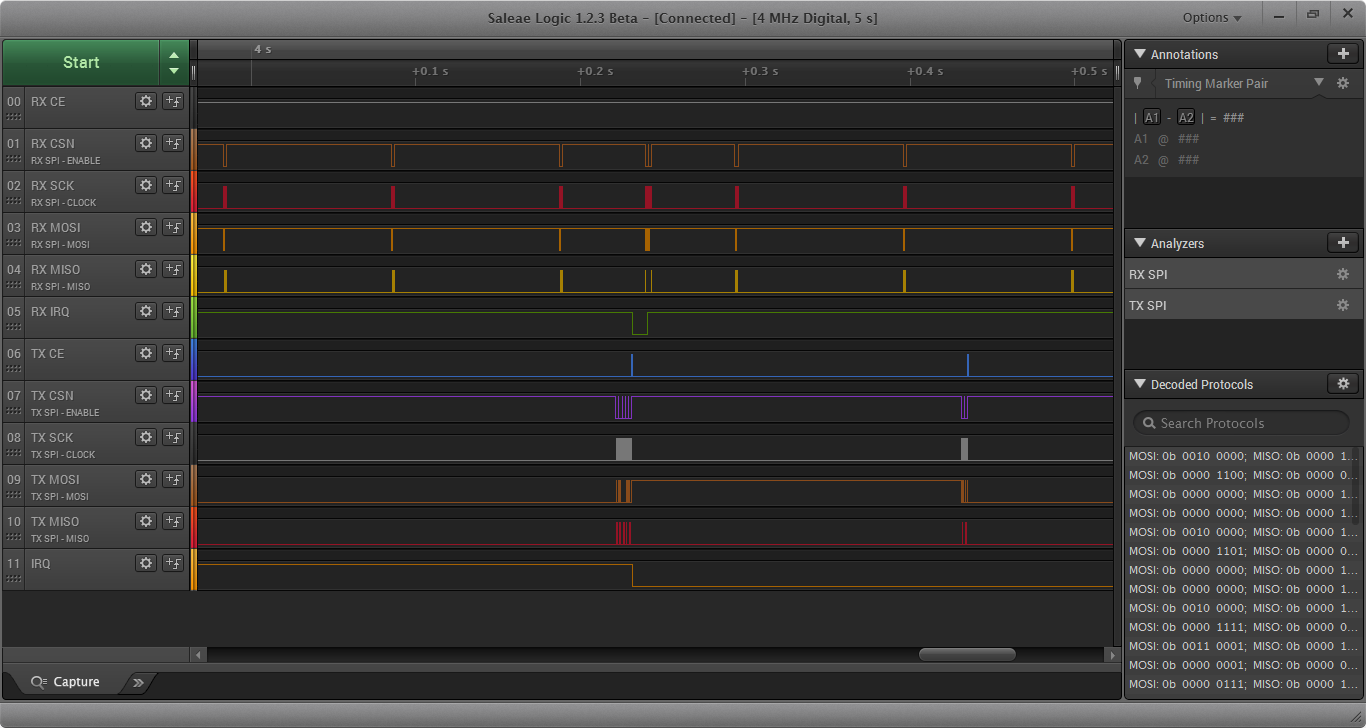
\includegraphics[width=0.75\linewidth]{images/30_08_2015_IRQ}}
    		\vspace{10pt}
    		
    		Here we can see that IRQ on the RX end drops low for one packet, however the IRQ on the TX end is low continuously after the first packet.\\
    		
    		\centerline{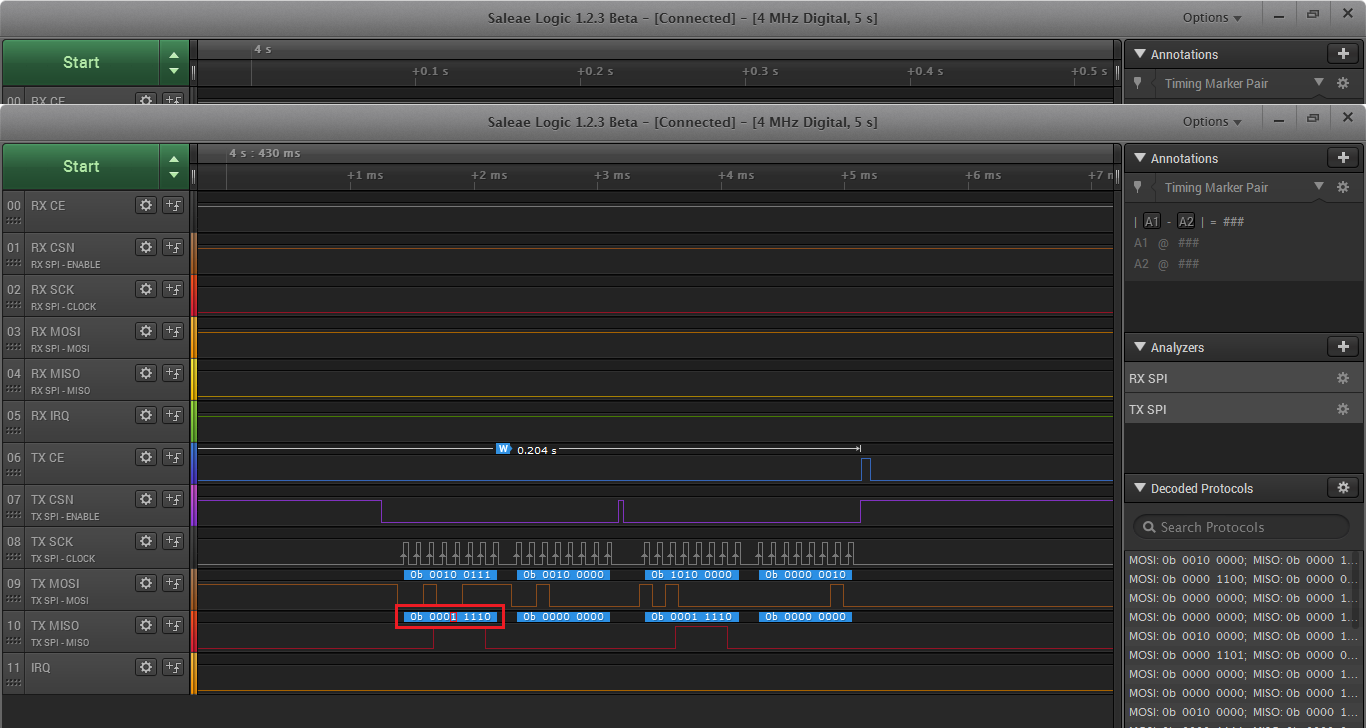
\includegraphics[width=0.75\linewidth]{images/30_08_2015_RTRM}}
    		\vspace{10pt}
    		
    		In this image you can see that the max retransmit \index{bit}bit has been set to one in the status byte. This means the \index{transmitter}transmitter has tried transmitting a index{byte}byte, but it didn't get any acknowledgment back - so it tried retransmitting. It's reached is max retransmit amount without any return signal, so it throws the MAX\_RT IRQ flag.\\
    		
    		To fix this I can either disable AUTO\_ACK on the TX, or enable AUTO\_ACK on the RX end.\\
    		
    		I ended up fixing the problem by disabling AUTO\_ACK on both RX and TX. This solution is not optimal as there is obvious \index{packet}packet drop between TX and RX - which the auto retransmit would normally fix. From now I'll be working on making this connection more \index{robust}robust (by enabling the autoack) and adding more features to my driver code.\\ 
    		
    		\centerline{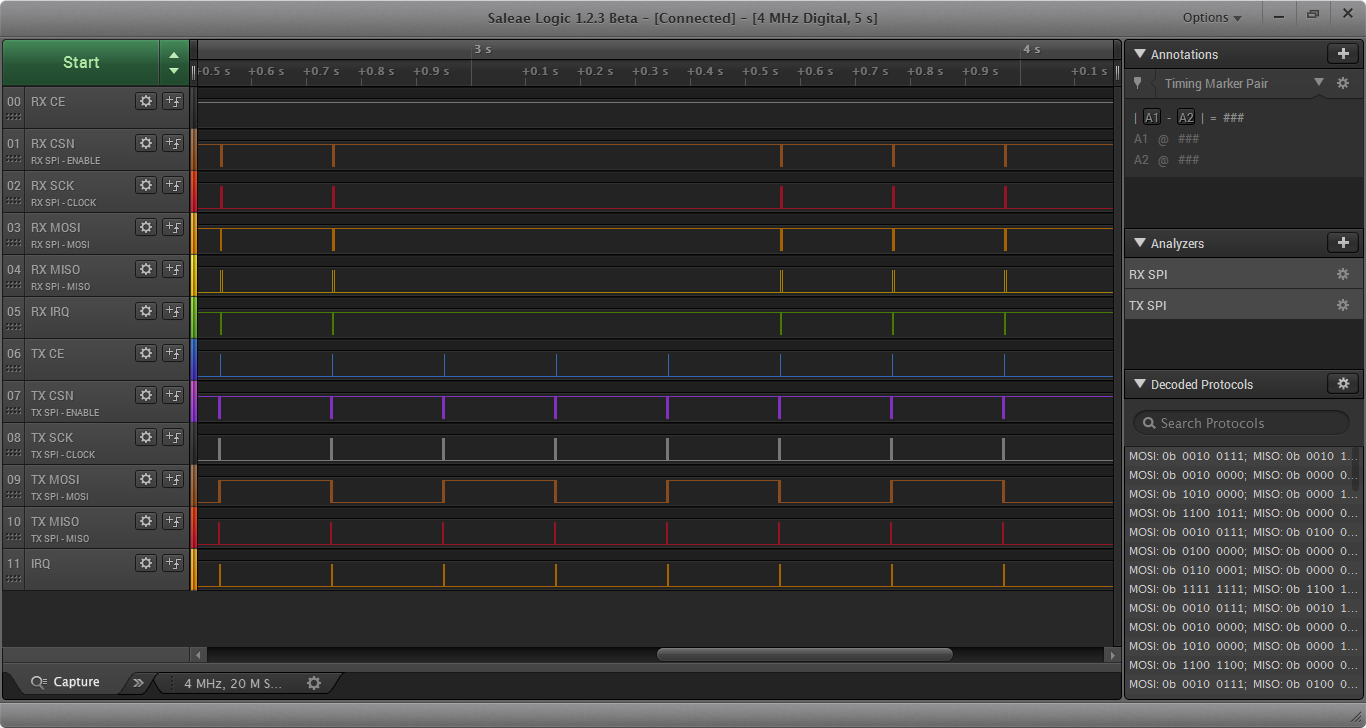
\includegraphics[width=0.75\linewidth]{images/30_08_2015_PKT_DRP}}
    		\vspace{10pt}
    		
    	\section{August 31st, 2015}
    	
    		I didn't do too much today. I've been picking out some songs for the \index{routine}routine, but nothing major yet. I have several \index{criteria}criteria I use when picking out songs. They either have to be well known (and loved), or have a good strong beat that people generally like. Secondly the section of the song I want to use has to be ~20s long, 40s max. If I have too much beyond this, I don't have enough time in the \index{routine}routine for other songs.\\
            
            \textbf{NOTE: }Also read \hyperref[sec:audio_selection]{Audio Selection}
    		
    		\textbf{Why do I use different songs?} Having not entered dance previously, and thus not being affected by the general mentality to only pick one song, I thought of having a mashup of multiple songs - inspired by this Britain's Got Talent performance:\\
    		
    		\url{https://www.youtube.com/watch?v=FP7wN301yjc}\\
    		
    		At \index{regionals}regionals I tried this out, and it was highly praised. It was commented that it showed that the robot could dance to a variety of \index{genres}genres. This effect was multiplied at regionals because of the variety of genre I was using (classical, pop, rock, etc). With a general mix of more contemporary songs this effect is lessened, but I feel that it provides variety to the routine.\\
    		
    		Beyond that, I took some time to find a suitable theme for my \index{website}website, which I hope to use to post information about my exploits on. I spent time experimenting with the "Freestyle" \index{rendering}rendering option in \index{Blender}Blender, in an attempt to make a logo/letterhead/headerimage. I was quite pleased with the results:\\
    		
    		\centerline{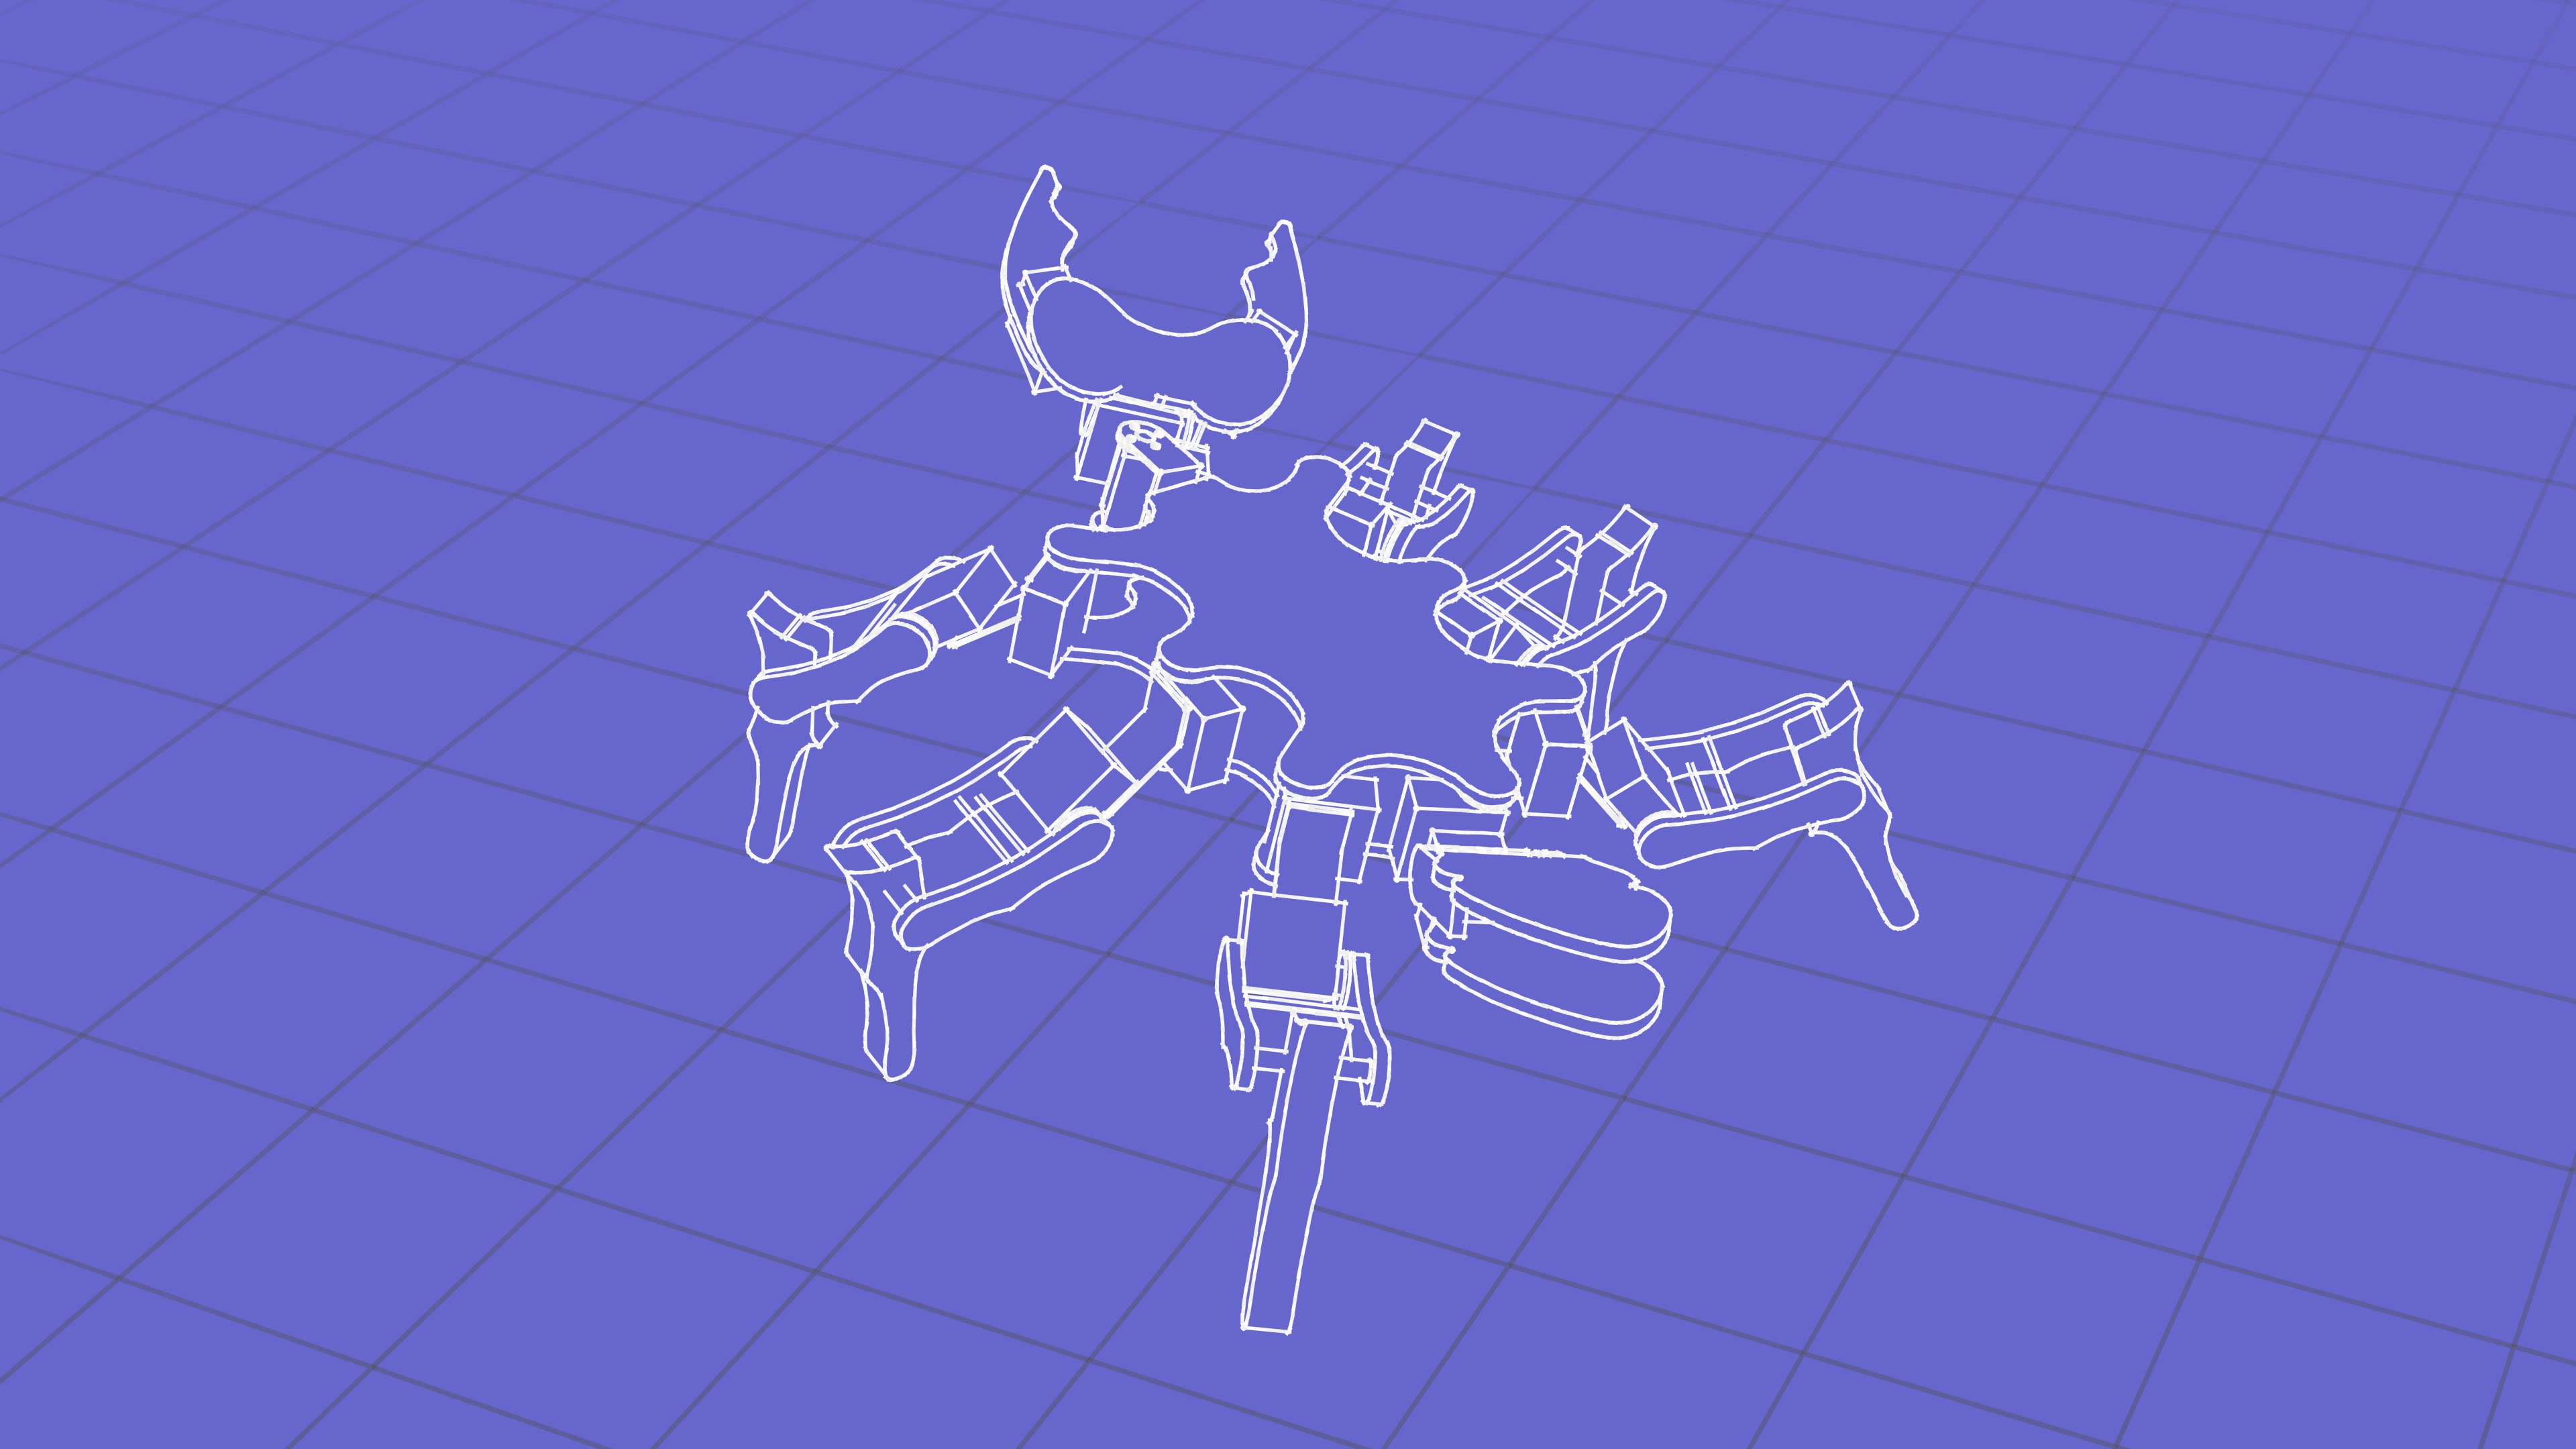
\includegraphics[width=0.75\linewidth]{images/blueprint_logo_4k}}
    		\vspace{10pt}
    		\centerline{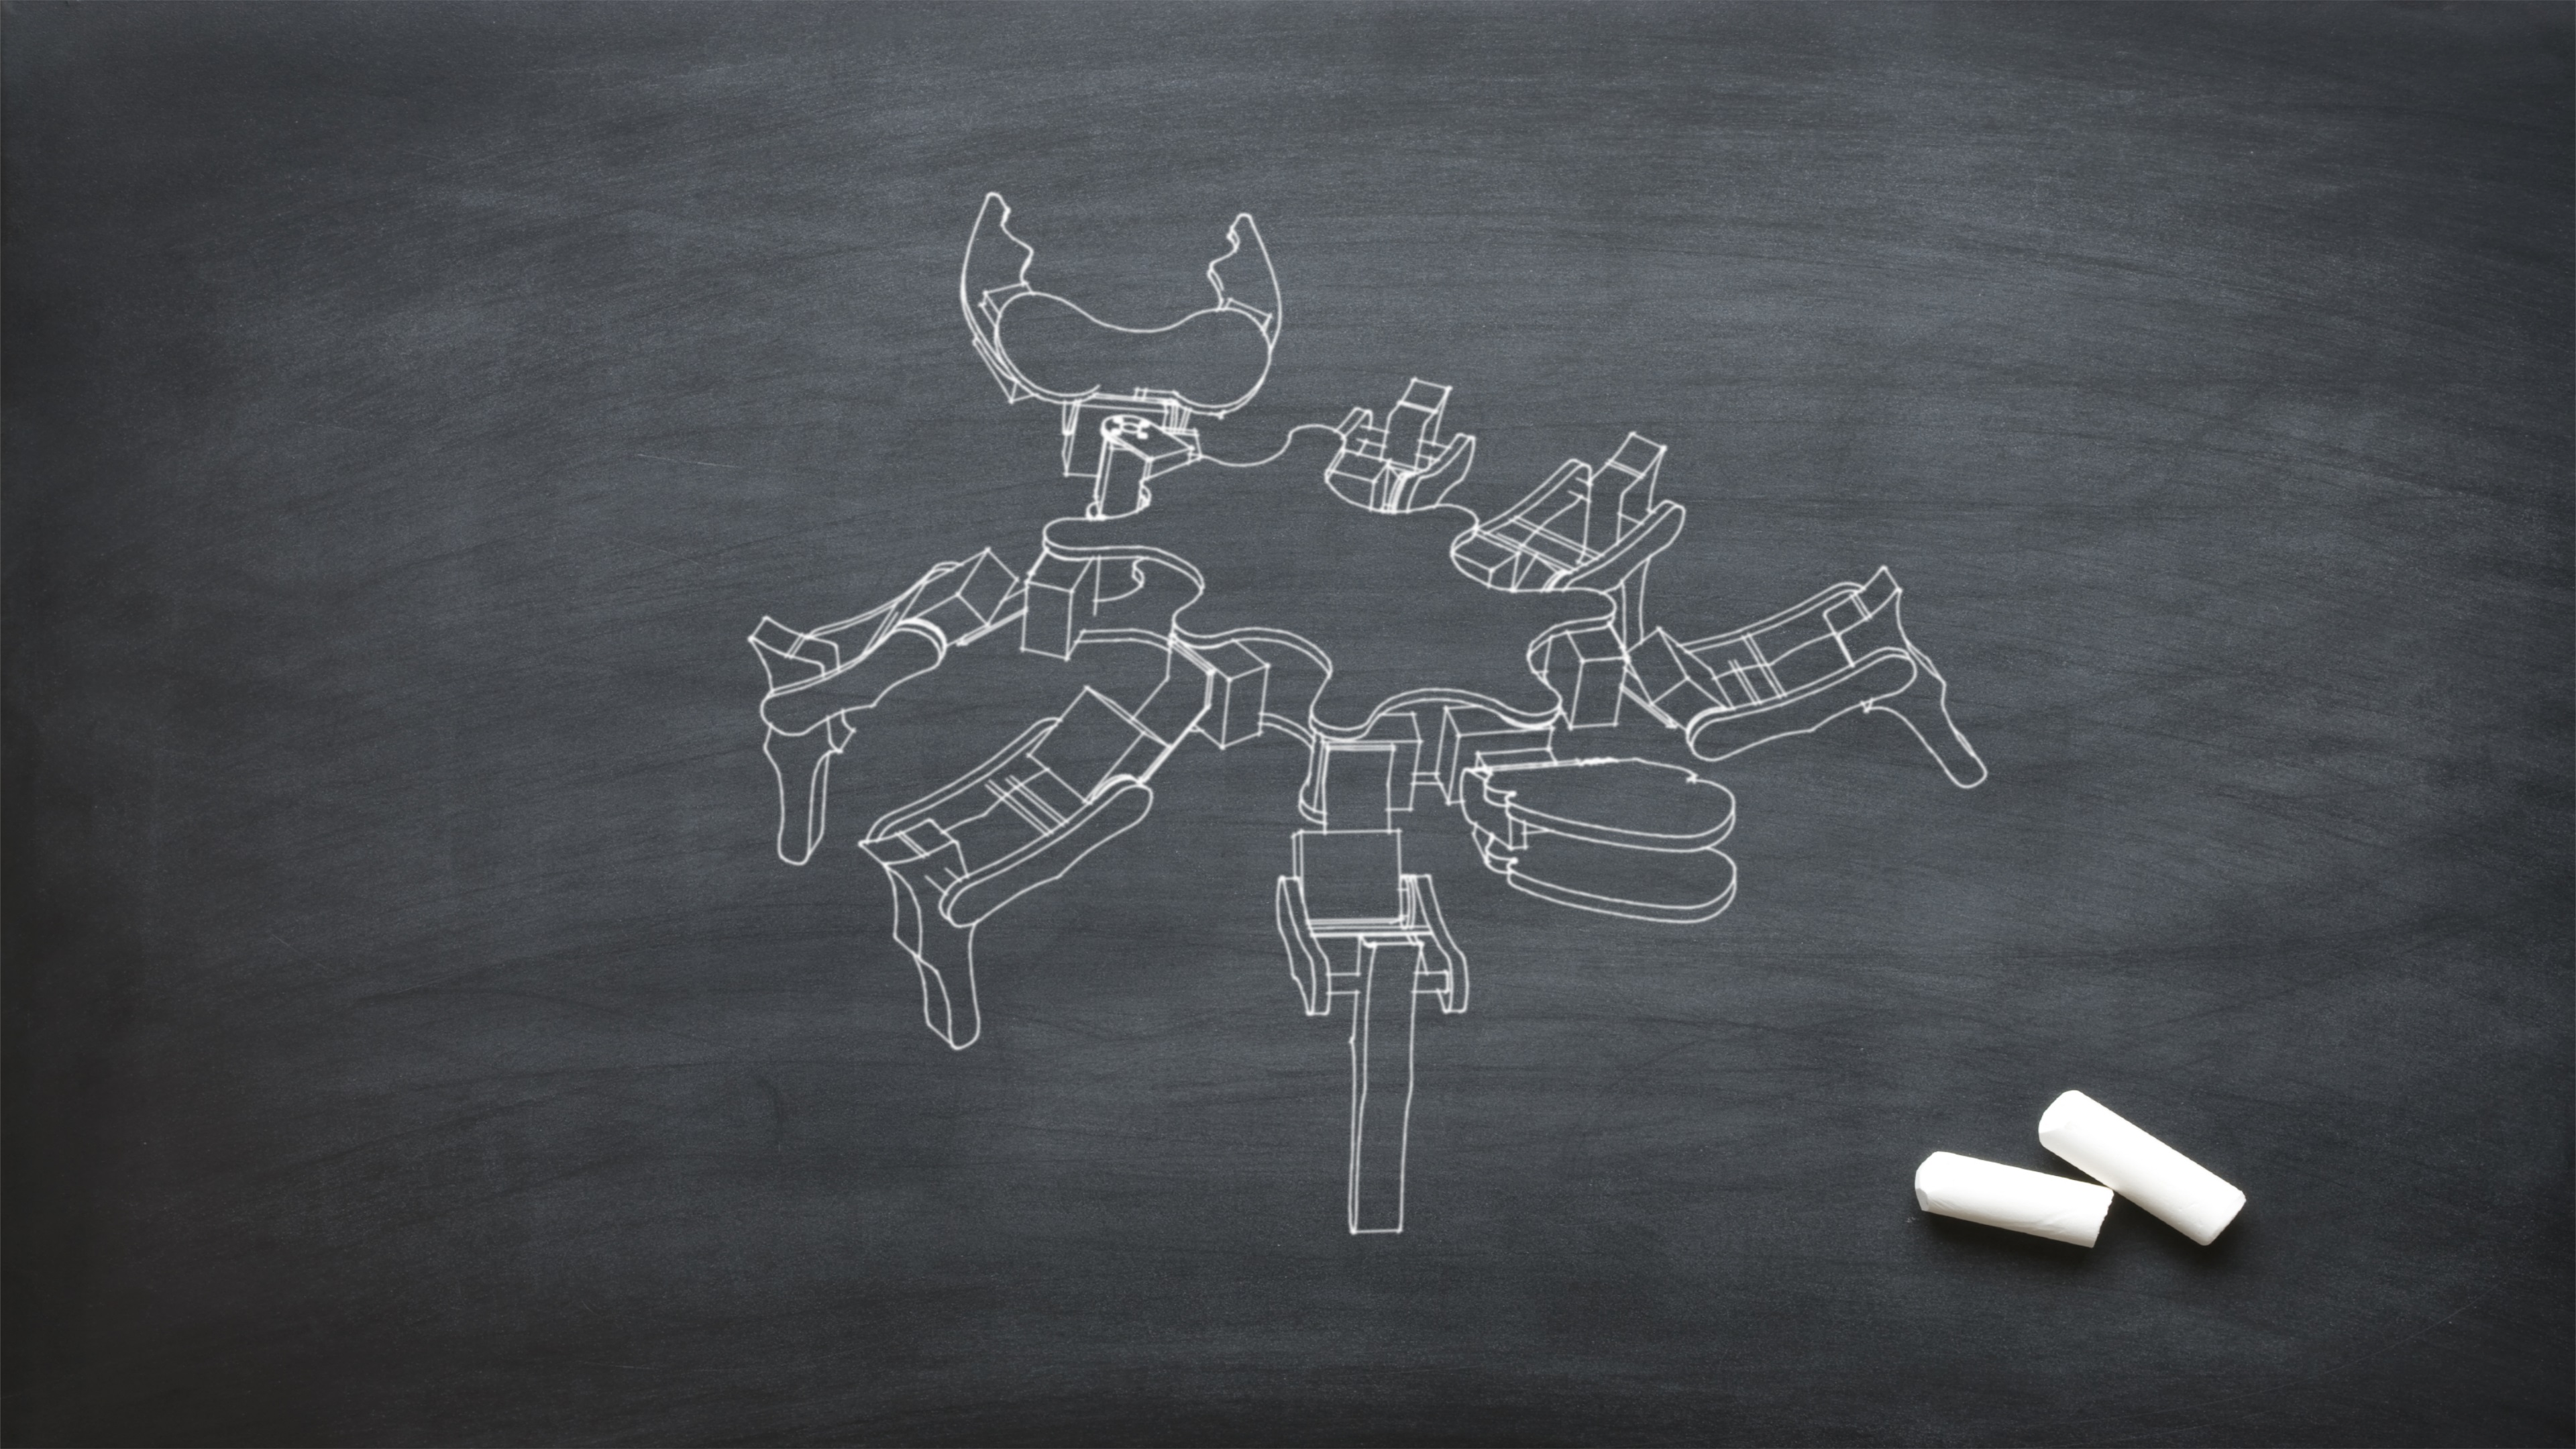
\includegraphics[width=0.75\linewidth]{images/chalkboard_logo_4k}}
    		\vspace{10pt}
    		
    		As I mentioned, I used the \index{freestyle}freestyle rendering option in blender. For the "blackboard" image I exported the lines generated by this function as an SVG, which I imported into \index{Inkscape}Inkscape, which I then used to superimpose onto a \index{blackboard}blackboard. I also modified the blur and opacity of said lines in Inkscape to give a "chalky" effect.\\